\begin{figure*}[h]                                                           
 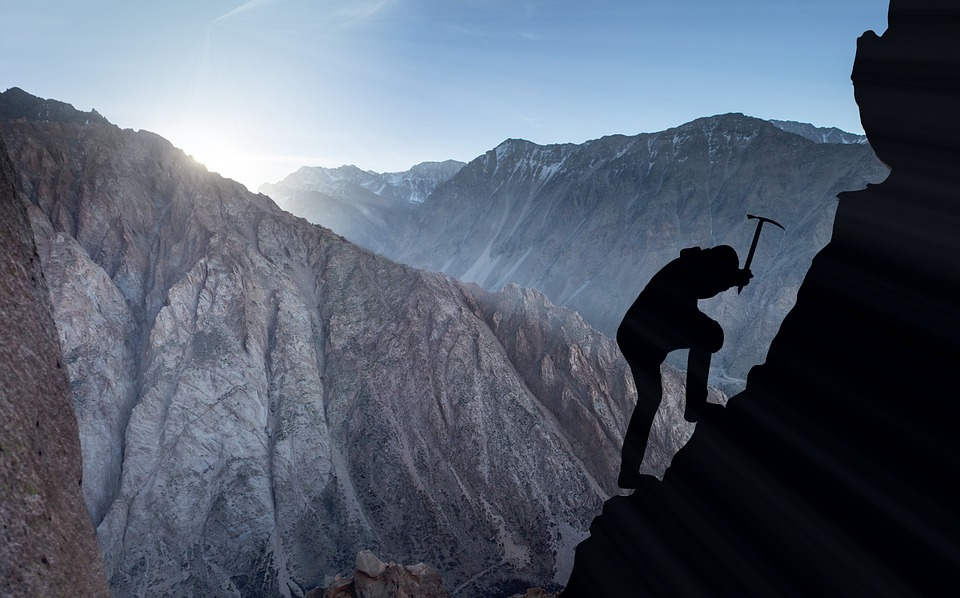
\includegraphics[width=\linewidth]{./media/images/summit}%
%  \scriptsize{\textsc{\\This is} the article main image caption.}
  \label{fig:editorial}%                                                 
\end{figure*}                                                                
\begin{quotation} 
\noindent\color{Sepia}{{\textit{\textbf{“Desire is the starting point of all achievement, not a hope, not a wish, but a keen pulsating desire which transcends everything.”}}}}\\[.5mm]
%remove following line space if you're tight on vertical room and need to fit on
%single page

\hfill\color{Sepia}{\small{\textendash \textsc{Napoleon Hill}}}
\end{quotation} 
\marginnote{Editor's note: margin notes in red signify links pointing to sites of reference}[2em]
%\lettrine[lines=3]{\color{BrickRed}I}{\enspace magine an afternoon outing filled
%  with discovery in detail.} What would it be like to explore a nature trail,
%museum, or even the area around Times Square where each turn presents new
%experiences of the 
\lettrine[lines=3]{\color{BrickRed}L}{\enspace ooking out across Willapa Bay's}
crystal blue waters I wonder about the rich history of this area. Was this
area\textemdash the place I am standing at this moment\textemdash used as a trade
route? Did Native Americans fish here? Could I be standing in the very spot
that a Willapa Chief once surveyed deciding the best course for his people? What
must it be like experiencing this place through the eyes of Natives going back
hundreds of years?

\marginnote{\href{https://en.wikipedia.org/wiki/Chinookan_peoples\#/media/File:Lewis_and_clark-expedition.jpg}{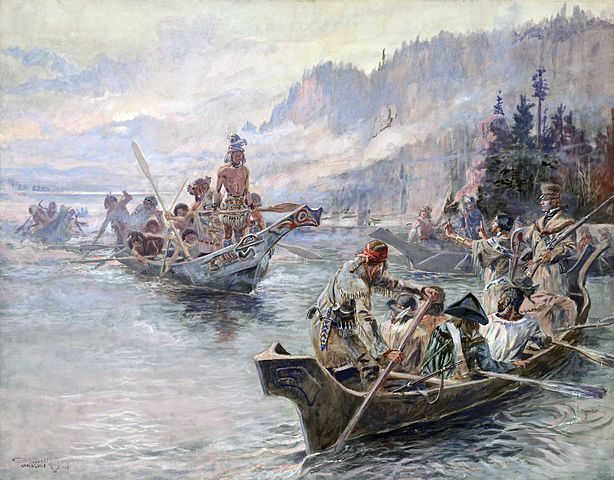
\includegraphics[width=\linewidth]{./media/images/lewis}\\Chinook people meet the Corps of Discovery on the Lower Columbia, October 1805}}[1em]
I approach a little further as my phone vibrates gently letting me know it's 
sensed that I've come to a place having significant import. I read the
Trail Guide's description of the place I am standing with a brief paragraph outlining
that yes, the \emph{Willapa} (or \emph{Willoopah}) tribe, an Northern
Athapaskan\textendash speaking people, did in fact use this very spot as a main
route between the Pacific Ocean 12 miles to the North and the Columbia River to
the South.

I'm no longer just walking along a trail, I'm also walking through time. I close my eyes
and imagine being there when the Chinook people meet the \emph{Corps of Discovery} on the Lower Columbia, near here, in 1805.

\section{limitless exploration}
Continuing along the trail I explore the area's geology, biology, and
wildlife. 
I learn that this area is a critical ``lung'' by which toxins created by water 
runoff is filtered making it
\marginnote{\href{http://portfolio.cooper.stevenson.name/tarlatt/tarlatt_slough_trail_feature_demo.mp4}{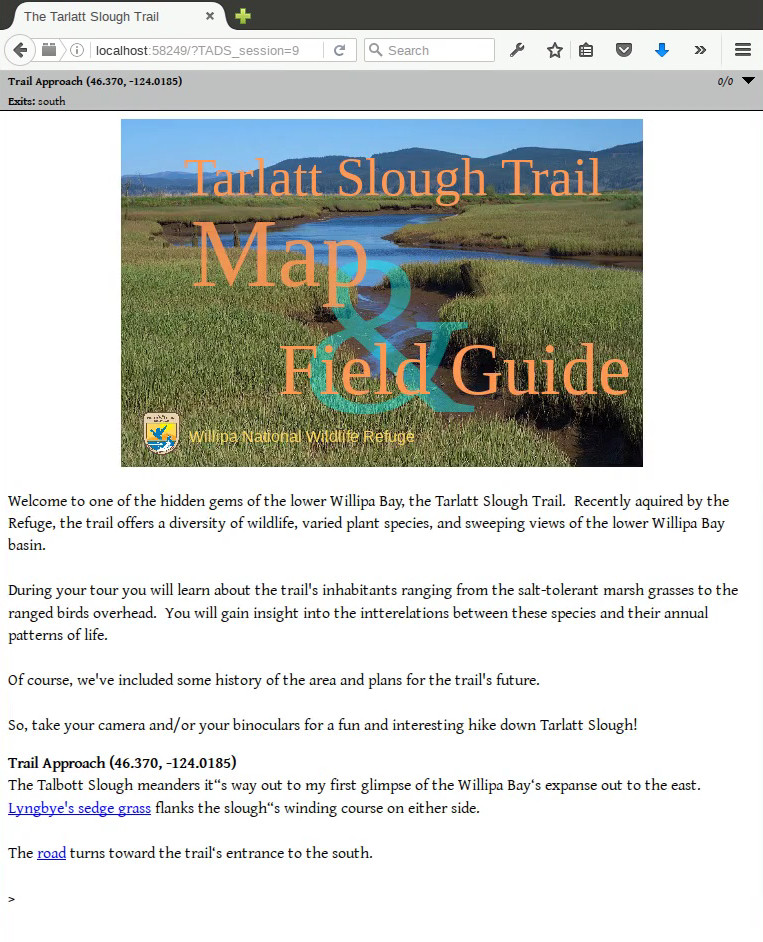
\includegraphics[width=\linewidth]{./media/images/tarlatt}\\Brief
    video showcasing \textsc{gps} enabled Interactive fiction's
    features}}[2em]possible for plankton to thrive giving way to higher forms of wildlife. I learn
that everything I see before me is a delicate balance; I learn of the efforts the
Wildlife Service is performing to keep it that way. I gain a better appreciation
for the area and learn that the term \emph{fragile ecosystem} is more than
mere phrasing; I learn \emph{why}.

\subsection{knowledge you can feel}
\noindent Parents or instructors may afford their children or a group of students impactful
learning experiences through an \texttt{\scriptsize{instructor}} mode (entered as a command
on the parent/instructor's tablet) 
while traveling along with a group of students.
\marginnote{Interlocutors may also \href{https://en.wikipedia.org/wiki/Citizen_science}{participate in Citizen Science} by recording natural findings through the \textsc{if} Tour Guide.}[-3em]
The instructor mode contains
supplemental information to help instructors guide or encourage students to explore areas
that are not obvious. Information imparted by the instructor is heard
by the students \emph{while the students physically interact with the topic at
  hand}. In a single command the instructor or parent is enabled to provide
their students tangible experiences covering a wider range of knowlege with increased depth.  

\subsection{economic benefit}
Interactive tours are not, of course, limited to natural trails. They may be
built for all manner of locations including museum
tours, tourist\textendash based main streets or as a guide for a battlefield
reenactments.
\marginnote{\href{http://www.marshsfreemuseum.com/}{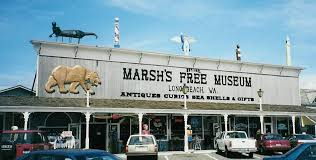
\includegraphics[width=\linewidth]{./media/images/marsh}\\Marsh's
    Free Museum}, in Long Beach Washington, offers all kinds of eclectic stuff including Jake, a
  ``half\textendash man half\textendash alligator.''}
Tourists walking down main street, for example, may learn of the area's
attractions (past and present) just across the street. Long Beach Washington,
for example, features Marsh's Free Museum. Marsh's is, I promise you, is the weirdest
``museum'' you've ever seen. Exhibits include turn\textendash of\textendash
the\textendash century parlor games, live hermit crabs, and ``Jake,'' a (as
legend has it) \emph{real} half\textendash man, half\textendash alligator.
The \textsc{gps\textendash} enabled tour tantalizes the would\textendash be
gawker of all the ridiculous indulgences awaiting inside.

\marginnote{Geocachers may also benefit from \textsc{gps} Interactive Fiction by
having the member solve a brain teaser before revealing the cache's final coordinates}[1em]
Designers can place site\textendash appropriate puzzles in the system for
exploration beyond the physical location. Perhaps an archaeological site is found where the
Interlocutor must figure out how to excavate a precious artifact without
damaging it. For this to work a  particular tool must be found. The reader has
just learned a) the importance of care in archaeology and b) an appreciation for
just how hard the archaeologist's task is. 

Your readers derive added benefit beyond the initial visit and may be passed to
friends and relatives through social media. This encourages others to visit as
the \textsc{if} work offers a preview of the destination from the comfort of
their living room. The shared version of
the work may even
offer embedded advertisements for travel packages and merchandise from the venue
itself or local businesses.

\section{Meaningful Experiences}
This issue if \emph{Discoverer's Digest} explores pushing the limits of
\textsc{if} beyond the screen and parser. The technical guide for enabling
\textsc{gps} in your Interactive Fiction gives a recipee for rich experiences in
the real world by combining the power of an interactive experience with the
sensory awareness of actually \emph{being there}.
\section{the best puzzles}
Brian Rushton systematically breaks down the underlying elements of puzzles
found in Interactive Fiction that help bring enjoyment to the medium. He answers
the questions, ``what are the parameters for good puzzles,'' ``how do I involve
the player,'' and ``what's at stake?''

\section{murder in the mail}
Finally, we've an interview with Felicity Banks, the author of several novels
including \emph{And Their Heroes Were Lost} and \emph{Attack of the Clockwork
  Army}.

Her new work, \emph{Murder in the Mail}, is a feelie story system in which cozy
crime stories are told via physical letters, objects, and high-quality art
prints physically mailed to the reader over several weeks. The reader is invited to guess the identity of the murderer and/or share clues on the forum.

\section{relax and enjoy}
As always, I hope you enjoy this eddition of \emph{Discoverer's Digest}; this
issue looks to be a dandy.

And please submit your news, story ideas, and comments by sending a personal email to \href{mailto:cooper@discdigest.xyz}{cooper@discdigest.xyz}. \\ \\

\noindent Happy Writing! \\ \\

\noindent \href{mailto:cooper@discdigest.xyz}{\textsc{D. Cooper Stevenson}}
